\documentclass[conference]{IEEEtran}

\usepackage{cite}
\usepackage{graphicx}
\usepackage{xcolor}
\usepackage{hyperref}
\hypersetup{colorlinks=true,linkcolor=black,citecolor=blue,filecolor=black,urlcolor=blue}
\graphicspath{{figures}}
\usepackage{caption}
\usepackage{subcaption}
\captionsetup[subfigure]{singlelinecheck=false, skip=0pt}
\usepackage{listings}
\renewcommand{\lstlistingname}{Algorithm}
\usepackage[binary-units=true]{siunitx}
\usepackage{csvsimple}
\usepackage{booktabs}
\usepackage{amsmath}

\usepackage{color,soul}
\newcommand{\TG}[1]{\color{blue}\textsc{From Tristan: }#1\color{black}}
\newcommand{\MD}[1]{\color{magenta}\textsc{From Mathieu: }#1\color{black}}
\newcommand{\HL}[1]{\hl{#1}}

\title{An Analysis of Performance Bottlenecks in MRI Pre-Processing}
\author{Mathieu Dugr\'e, Yohan Chatelain, Tristan Glatard\\Department of Computer Science and Software Engineering, Concordia University, Montreal, QC, Canada}

\begin{document}
\maketitle

\begin{abstract}
	Magnetic Resonance Image (MRI) pre-processing is a critical step for neuroimaging analysis. However, the computational cost of MRI pre-processing pipelines is a major bottleneck for large cohort studies and some clinical applications. While High-Performance Computing (HPC) and, more recently, Deep Learning have been adopted to accelerate the computations, these techniques require costly hardware and are not accessible to all researchers. Therefore, it is critical to understand the performance bottlenecks of MRI pre-processing pipelines to improve their performance. Using Intel VTune profiler, we characterize the bottlenecks of several commonly used MRI-preprocessing pipelines from the ANTs, FSL, and FreeSurfer toolboxes. We found that few functions contribute to most of the CPU time, and that linear interpolation is the largest contributor. Data access is also  a substantial bottleneck. Last, we identified a bug in the ITK library that impact the performance of ANTs pipeline in single-precision and a potential issue with the OpenMP scaling in FreeSurfer recon-all. Our results provide a reference for future efforts to optimize MRI pre-processing workflows.
\end{abstract}

\section{Introduction}
% Computational bottleneck
Pre-processing of Magnetic Resonance Imaging (MRI) data is a critical step in neuroimaging. Although established pre-processing pipelines exist, they commonly require expensive computation and produce large output and intermediate data. \HL{These are a well-known challenges to study large subject cohorts in neuroimaging.} Moreover, the execution time of pipelines can hinder clinical applications where timely data analysis is needed. Therefore, the neuroimaging community is constantly seeking ways to improve the performance of MRI pre-processing pipelines.

% HPCs
Researchers broadly adopted High Performance Computing (HPC) to accelerate the MRI processing of large cohorts \HL{leveraging} a large number of CPU cores and high-bandwidth memory to process subjects in parallel. However, \HL{it can be challenging to run HPCs in developing countries due to power restrictions, national network infrastructure, and lack of training and funding}~\cite{NRG-SC23}. \HL{Similarly, researcher use cloud computing, but it requires expertise to setup, can be costly for large studies, and} data transfer can be slow and might be impossible due to ethic concerns related to human data. \HL{In both cases, limitation from the parallel efficiency of the pipeline can lead to under-utilization of the available resources.}

% DL
In recent years, Deep Learning (DL) has shown promising results in MRI pre-preprocessing. For example, tools such as SynthMorph~\cite{Hoffmann2022-hu}, SynthSeg~\cite{Billot2023-vp}, SynthSR~\cite{Iglesias2023-bp}, and SynthStrip~\cite{Hoopes2022-ms} were integrated into FreeSurfer~\cite{Fischl2012-cx} to provide Deep Learning alternatives to traditional algorithms\HL{, providing faster runtime.}
% Moreover, a study~\cite{Pepe2023-dm} showed that the results generated by SynthMorph are numerical more stable than those from FreeSurfer.
However, training a DL model requires large amount of data and specialized hardware, and is computationally expensive. Additionally, \HL{their results} can be challenging to interpret, explaining the slow adoption of DL in MRI pre-processing.

% Alternative solutions
\HL{These techniques require costly hardware to be effective, which can be unacessible to underrepresented researchers.} Alternatively, improved algorithm designs, compression techniques, or reduced- and mixed-precision techniques could provide substantial performance improvements but require substantial effort to implement. Therefore, it is critical to understand the performance bottleneck of MRI pre-processing pipelines to improve their performance.

% - No comprehensive study of the performance bottleneck of MRI pre-processing.
\HL{To the best of our knowledge, this is the first study that} characterize the computational cost of several commonly adopted MRI pre-processing pipelines. The results of our analysis serve as a reference for future efforts to optimize MRI pre-processing workflows.

% - Focus on MRI pre-processing.
MRI is a standard tool used by neuroscientists to perform clinical diagnosis and for researchers to develop a better understanding of the brain. Three main MRI modalities exist: structural MRI (sMRI), functional MRI (fMRI), and diffusion MRI (dMRI). While other modalities such as electroencephalography (EEG), computed tomography (CT), and positron emission tomography (PET) exist, we focus on MRIs for their broad adoption and non-invasiveness. Moreover, MRI data analysis is challenging due to computationally expensive pre-processing and large output and intermediate data size.

% - Pipelines
Neuroscientists developed various toolboxes to tackle the challenging task of pre-processing MRI data. We focus on the commonly accepted fMRIPrep~\cite{Esteban2019-bl} workflow as it a comprehensive pre-processing pipeline for both sMRI and fMRI. fMRIPrep combines several pipelines to produce a complete pre-processing workflow. We also study its sub-workflow separately to provide a finer grain analysis of the performance bottleneck.

% - data: OpenNeuro ds004513
% We use the OpenNeuro ds004513 v1.0.2 dataset~\cite{ds004513:1.0.2}. We chose this dataset for its wide range of age and equal distribution of biological sex. Using a diverse dataset should help to prevent findings of potential performance bottleneck associated to a specific population. \TG{Move this to methods}

% - VTune profiler
To profile the pipelines, we use the Intel VTune profiler~\cite{vtune-profiler}. The VTune profiler is a multi-language profiler with low performance overhead and provides information of functions at runtime level. We profile the application using \HL{-- single-threaded and 32 threads to simplify the analysis and study the the multi-threading performance, repsectively}. We aggregate subjects' results for each pipeline to obtain an average performance profile. We compiled each application with debug information to obtain human readable information on function and module names in VTune.

\section{Materials \& Methods}
\subsection{Pipelines}
We study the performance bottleneck of fMRIPrep; a commonly used fMRI and sMRI pre-processing workflow. First, we profile the entire workflow to obtain a coarse view of the workflow's performance. Furthermore, to characterize the performance at a finer grain, we profile the sub-workflows of fMRIPrep: ANTs brainExtraction, ANTs registrationSyN~\cite{Avants2008-ea}, FreeSurfer recon-all~\cite{Dale1999-wu}, FSL FAST~\cite{Zhang2001-hx}, FSL FLIRT~\cite{Jenkinson2002-od,Jenkinson2001-eu,Greve2009-dw}, and FSL MCFLIRT~\cite{Jenkinson2002-od}. We omitted some sub-workflows of fMRIPrep as they were not compatible with our dataset \TG{add a few words to explain why}. \TG{Information is missing to explain what is the statistical analysis in fMRIPrep. Likewise, it's unclear what ANTS registration, FSL Flirt, etc are and how they are combined in fMRIPrep. This section should start with a higher-level overview of fMRIPrep. You should also explain that fMRIPrep's building blocks are widely used in neuroimaging.} Moreover, the statistical analysis of the fMRIPrep workflow is not computationally expensive and is not the focus of this paper.

We use the default parameters for fMRIPrep and most of the sub-workflows. However, for FreeSurfer recon-all, we mimic the fMRIPrep specific 3 stages workflow \TG{This is cryptic, it needs more context.}.

We profile both the single and double precision version for ANTs registrationSyN and ANTs brainExtraction. ANTs uses ITK templates to implement the single precision alternative. \TG{You should re-order this paragraph as follows: (1) ANTs registration has two implementations, a double precision one and a single precision one. (2) This is actually coming from ITK. (3) We benchmark both implementations.}

\subsection{Data}
To ensure that our performance profiles are inclusive of different populations, we used data with a wide range of age and equal distribution of sex. We used the the OpenNeuro ds004513 v1.0.2 dataset~\cite{ds004513:1.0.2}. The anatomical, functional, and diffusion data from 20 health individuals was acquired from two different cohorts. The within-subject cohort has nine participants (mean age=43~yrs, std=7~yrs; 4 females) with two session: eyes open and eyes closed. The replication cohort has eleven participants (mean age=27~yrs, std=5~yrs; 6 females) with only the eyes open session. We profiled the application using both cohorts and the eyes open session, unless explicitly specified \TG{is it ``explicitly specified'' anywhere? If not, remove this.}.

\subsection{Profiling}
Profiling MRI pre-processing pipelines \TG{the terms pipelines, workflfows, applications are used interchangeably, let's harmonize and use only 1 term (I don't mind which one)} raises a few challenges. Neuroimaging pipelines use several programming languages including \textit{C}, \textit{C++}, \textit{Fortran}, \textit{Matlab}, and \textit{Python}, with several pipelines utilizing a combination of multiple languages. Pipelines are generally complex and computationally expensive.

The Intel VTune profiler addresses these challenges by offering multi-language support, low performance overhead, and information of functions at runtime level. However, common profiling challenges remain. Profilers require source code to be compiled with debug symbols to report interpretable information about the different functions and modules. Moreover, different input data can substantially impact the performance results due to conditional branching in the application and convergence thresholds. We discuss our approach to these challenges in the next section.
\MD{TODO Cite effect from varying input data on numerical stability and reduced precision. Ask yohan for references}
		
First, to obtain human readable information on function and module names in VTune, we re-compiled each pipeline with debug information in a Docker image. For use on HPC systems, we created Apptainer~\cite{Kurtzer2017-bu} images using Docker2Singularity\footnote{\href{https://github.com/singularityhub/docker2singularity}{https://github.com/singularityhub/docker2singularity}} \lstlistingname~\ref{alg:vtune_example} \TG{Could this be called a listing rather than an algorithm?} illustrates the profiling of a pipeline by mounting the VTune binary to the Apptainer image during execution.

\begin{minipage}{\linewidth}
	\lstinputlisting[
		language={sh},
		caption={Profiling an application within a Apptainer container, using VTune profiler.},
		captionpos=b,
		label=alg:vtune_example,
		numbers=left,
		frame=single,
		basicstyle=\footnotesize,
		numbersep=5pt,
		numberstyle=\tiny\color{gray},
		rulecolor=\color{black},
		tabsize=2,
	]{vtune-example.sh}
\end{minipage}
				
Second, we aggregate the profiling results of each pipeline across all subjects to obtain an average performance profile. The Pareto principle is a power law which states that 80\% of the effects come from 20\% of the causes. We hypothesize that the Pareto principle applies to the performance of MRI pre-processing pipelines, which is consistent with the literature~\cite{Kukunas2015-jd}. Therefore, for fine-grained analysis, we only study the functions with the largest contribution to CPU time, up to 80\% cumulative total runtime of the application \TG{This discussion on Pareto principle should be moved to the results section}. This heuristic allows us to focus our efforts on the performance critical sections of a pipeline. We report the mean and standard deviation of the execution time for those functions.
			
Last, we profile the application using two threading configuration: single-threaded and 32 threads. The single-threaded approach simplifies the analysis and limits the potential overhead from I/O on the profiling. 
The 32-thread approach uses all available CPU cores from a compute node of our infrastructure to study the multi-threading performance of the application. This is a more realistic usage for the user of the application.
			
Before profiling each application, we transfer the input data from the shared file system to the compute node. After profiling, we transfer back the output to the shared file system. This limits profiling variability due to I/O contingency.
			
The data generated by the VTune profiler is written to a shared file system, for administrative reasons. In principle, this could increase the profiling overhead. However, in practice there is no impact since the data generated by the VTune profiler is very small and is not written on the same file system as data produced by the applications.
			
\subsection{Metrics Definition}
VTune provides several metrics to characterize the performance of an application.  The makespan is the elapsed time from the start to the end of the application. The CPU time refers to the total time spent by the CPU, across all cores, to execute the application. 

\begin{figure*}[ht]
	\noindent
	\begin{minipage}
		{0.5\textwidth}
		\begin{align*}
			C & = CPU\_CLK\_UNHALTED.THREAD                \\
			S & = CYCLE\_ACTIVITY.STALLS\_LDM\_PENDING     \\
			O & = CYCLE\_ACTIVITY.STALLS\_L1D\_PENDING     \\
			T & = CYCLE\_ACTIVITY.STALLS\_L2\_PENDING      \\
			W & = MEM\_L3\_WEIGHT                          \\
			H & = MEM\_LOAD\_UOPS\_RETIRED.LLC\_HIT        \\
			R & = MEM\_LOAD\_UOPS\_MISC\_RETIRED.LLC\_MISS \\
			M & = \frac{W \times R}{H + R}                 \\
			N & = \frac{H}{H + W \times R}                 
		\end{align*}
	\end{minipage}
	\begin{minipage}
		{0.5\textwidth}
		\begin{align}
			\%~Memory~Bound & = \frac{S}{C} \times 100          \\
			\%~L1~Bound     & = \frac{S - O}{C} \times 100      \\
			\%~L2~Bound     & = \frac{O - T}{C} \times 100      \\
			\%~L3~Bound     & = \frac{T \times N}{C} \times 100 \\
			\%~DRAM~Bound   & = \frac{T \times M}{C} \times 100 
		\end{align}
	\end{minipage}
	\caption{Intel performance monitoring events and derived memory metrics}
	\label{fig:memory-metrics}
\end{figure*}	
The memory bound metrics counts the number of cycles where the CPU is starved while waiting for in-flight memory demand load. L1 bound occurs when a demand load stall some CPU cores although the data already reside in L1 cache. Similarly, L2, L3, and DRAM bound occurs when a demand load stall the CPU and there is a cache miss in the previous level of cache, but the data reside in the L2, L3, and DRAM respectively. The store bound occurs when a store operation stall the CPU. Figure~\ref{fig:memory-metrics} shows the monitoring events and equation to derive the metrics defining the memory bound characterization~\cite{Intel2006-lc} \TG{This figure should go to appendix, it's not critical to the understanding of the paper}. We use the convention from~\cite{Kukunas2015-jd} for the equations.
			
The difference between the memory bound value and the sum of the other metrics represent the percentage of CPU starvation while waiting from data absent from all cache level, that is, when the data is being fetched from disk.
			
\subsection{Infrastructure}
We used the \textit{Slashbin cluster} at Concordia University. The compute nodes are configured with two 16-core Intel(R) Xeon(R) Gold 6130 CPU @ \SI{2.10}{\giga\hertz}, \SI{250}{\gibi\byte} of RAM, \SI{126}{\gibi\byte} of tmpfs, six \SI{447}{\gibi\byte} SSDs with the XFS file system (no RAID enabled), Rocky~Linux~8.9 and Linux kernel \textit{4.18.0-477.10.1.el8\_lustre.x86\_64}.
			
\section{Results}
In this section we present the aggregated profiling data obtained with VTune. First, we present a performance overview of the pipelines. We then analysis specific hotspots in the pipelines. Unless specified explicitly, we only present the profile data from using 1-thread since the results from 32-threads are similar.
			
\subsection{CPU time distribution across functions was long tailed}
Figure~\ref{fig:long-tail-distribution} shows that 80\% of the total CPU time was spent in less than 1.5\% of the function across all pipelines. While consistent with the Pareto principle, the distribution of the functions' CPU time does not follow a Pareto distribution. We plotted the distribution of the functions' CPU time on a log-log scale and found it to be closer \TG{``closer'' is too vague: is it well approximated by a Zipf's law? Can you provide a p-value of this claim?} to a Zipf's law distribution with exponent $\alpha=1.8$. \TG{Add a few sentences to explain why this is interesting.}

\begin{figure}[ht]
	\centering
	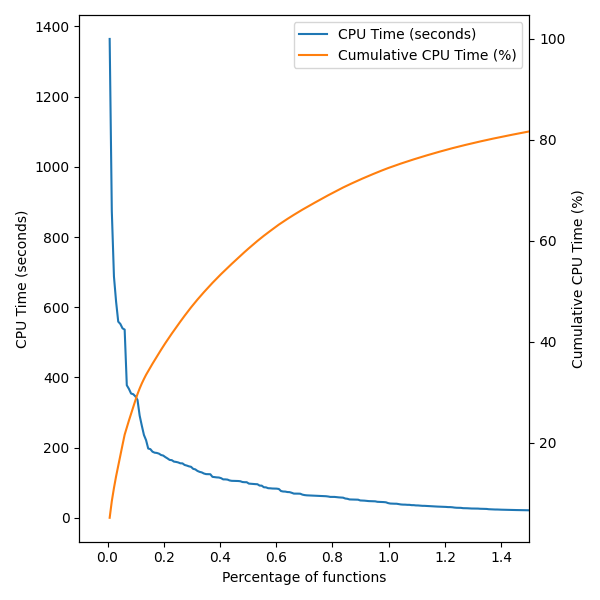
\includegraphics[width=\linewidth]{figures/global-longtail.png}
	\caption{Distribution of the functions' CPU time. The left y-axis shows the average total CPU Time spent in a function, while the right y-axis show the cumulative CPU time percentage. The x-axis percentage of functions ordered by decreasing CPU time. The data includes all functions from all pipelines. }
	\label{fig:long-tail-distribution}
\end{figure}
				
\subsection{Makespan: A performance overview}
Figure~\ref{fig:makespan-1thread} depicts the total time elapsed from the start to the end of each pipeline; i.e. makespan. There is a significant difference between the makespan of different applications. This is expected as the pipelines perform different tasks. The standard deviation is nearly null for all pipelines, except for FreeSurfer recon-all which as a small variation. Overall, this shows that the input data does not substantially affect the makespan of those pipelines. \TG{not sure what to make from this result, I don't find it particularly noticeable, I think I would omit it.}
			
\begin{figure}[t]
	\centering
	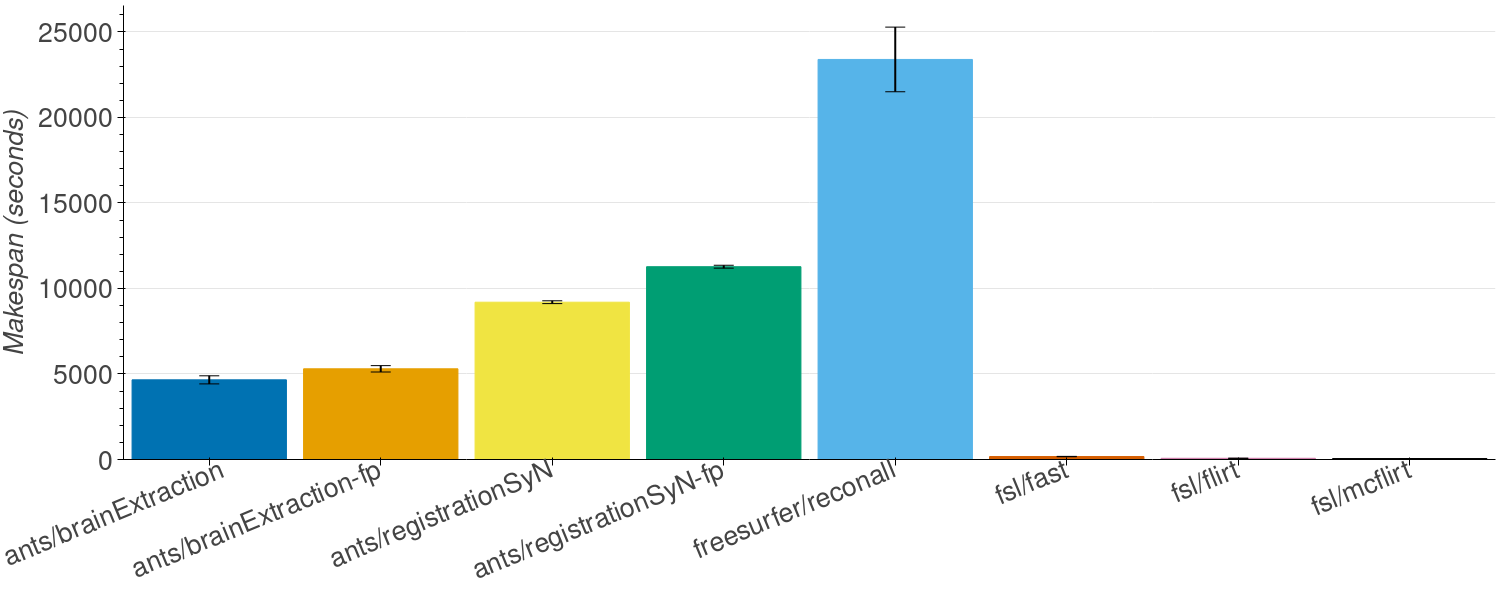
\includegraphics[width=\linewidth]{figures/makespan-1thread.png}
	\caption{Average makespan of the pipeline while using 1-thread. The error bars show the standard deviation. \TG{Font size in the figure is too small, it should be similar to the caption font size}}
	\label{fig:makespan-1thread}
\end{figure}
			
\subsection{Impact of Memory Bounded Functions}
Table~\ref{extab:memory-bound} shows that fetching data from disk is the main source of cycles where the CPU is starved \TG{I don't see disk in table 1}. Following, the L1 bound has the highest cache-level contribution to the memory bound of the pipelines. ANTS pipelines have the highest L1 bound, followed by FreeSurfer recon-all and FSL MCFLIRT. L2 and L3 bound is low for all pipeline, although highest for FreeSurfer recon-all. The DRAM bound is high for both FSL FLIRT and FreeSurfer recon-all, followed by ANTS brainExtraction in single and double precision. Store bound is low for all pipelines. We note an interesting relationship between the low L1 bound and the high DRAM bound of FreeSurfer recon-all and FSL FLIRT, compared to the other pipelines. \TG{Add discussion: what is interesting about this result?}
			
\csvnames{csvcol}{1=\pipeline, 2=\mem, 3=\la, 4=\lb, 5=\lc, 6=\dram, 7=\store}
\csvstyle{memory_bound}{
	tabular = |r|c|c|c|c|c|c|,
	table head = \hline Pipeline &  \% Memory Bound &  \% L1 Bound &  \% L2 Bound &  \% L3 Bound & \% DRAM Bound & \% Store Bound\\\hline\hline,
	late after line = \\\hline,
	respect all,
	csvcol
}
\begin{table*}[ht]
	\centering
	\csvreader[memory_bound]{tables/memory_bound.csv}{}
	{\pipeline & \tablenum[round-precision=2]{\mem} & \tablenum[round-precision=2]{\la} & \tablenum[round-precision=2]{\lb} & \tablenum[round-precision=2]{\lc} & \tablenum[round-precision=2]{\dram} & \tablenum[round-precision=2]{\store}}
	\caption{Impact of data load on stalled CPU cycles. The values are the summation of the metric weighted by each function CPU time. This represent the percentage of the total CPU time stalled by each metrics. We show the average value across all subjects execution with one thread.}
	\label{extab:memory-bound}
\end{table*}
			
\subsection{Main Bottleneck: Linear Interpolation}
Table~\ref{extab:interpolation} shows that interpolation (or convolution) is a critical part for all pipelines, except FreeSurfer recon-all. For those pipelines, interpolation contributes between 32.20\% to 62.70\% of the total CPU time. Overall, the number of functions using interpolation is low with less than 20 in each applications. In other words, few interpolation functions are contribute to a large portion of the CPU time. \TG{This should be moved up in the results, I think right after Figure 2, as this is one of the most interesting results.} \TG{Add a few sentences to explain why this is interesting.}
% There seems to be few  the stages from recon-all: https://surfer.nmr.mgh.harvard.edu/fswiki/recon-all (see section "Manual-Intervention Workflow Directives": stages 1-31)
			
\csvnames{csvcol}{1=\pipeline, 2=\nfunc, 3=\cputime}
\csvstyle{interpolation}{
	tabular = |r|c|c|,
	table head = \hline Pipeline & \# of functions & \% CPU Time \\
	& with interpolation & from interpolation\\\hline\hline,
	late after line = \\\hline,
	respect all,
	csvcol
}
\begin{table*}[ht]
	\centering
	\csvreader[interpolation]{tables/interpolation.csv}{}
	{\pipeline & \nfunc & \tablenum[round-precision=2]{\cputime}}
	\caption{Contribution of interpolation to the applications' total CPU time. The percentage is the average sum of CPU time of functions using interpolation. The data includes all functions; not only the top 80\% of the CPU time.}
	\label{extab:interpolation}
\end{table*}
						
						
\subsection{ANTS: Single vs. Double Precision}
Figure~\ref{fig:makespan-ants} shows the makespan of ANTS brainExtraction and ANTS registrationSyN in double and single precision. For both pipelines, the makespan is significantly higher in single precision. This is unexpected, as the floating-point arithmetic operations are supposed to be faster in single precision~\cite{Wang2018-jv}.

\begin{figure}[ht]
	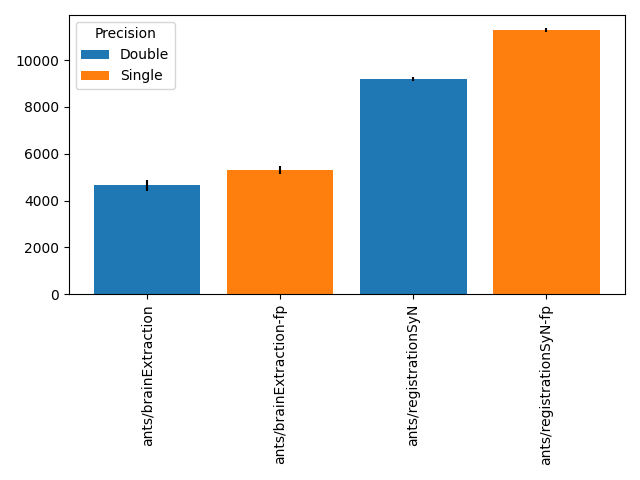
\includegraphics[width=\linewidth]{figures/makespan-ants.png}
	\caption{Comparison of makespan between double (blue) and single (orange) precision for ANTS brainExtraction and ANTS registrationSyN.}
	\label{fig:makespan-ants}
\end{figure}
			
The number of iteration between both version of ANTS registrationSyN is similar. In fact, for the latest two stages, they were the same across all but one execution. However, The single precision version of ANTS registrationSyN took longer per iteration than the double precision version (Figure~\ref{fig:mean-time-per-iteration-ants}). Therefore, the slowdown is not due to the convergence of the algorithm, but rather the execution time for each iteration. \TG{This is too inconclusive, you should give all the details here.}

\begin{figure}
	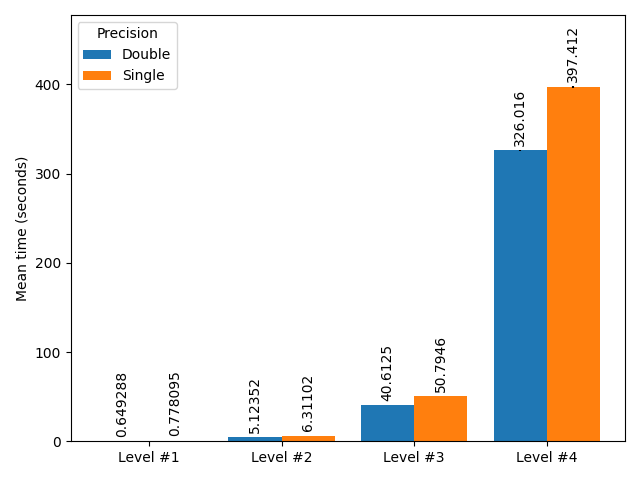
\includegraphics[width=\linewidth]{figures/ants-registrationSyN-iteration-mean.png}
	\caption{Mean time per iteration for ANTS registrationSyN in double and single precision. Only the SyN Registration stage is shown as the two earlier stage were near zero time. The error bars show the standard deviation.}
	\label{fig:mean-time-per-iteration-ants}
\end{figure}
						
\subsection{FreeSurfer: Thread-Synchronization}
Figure~\ref{fig:hotspots-freesurfer-reconall} shows a significant difference in the pipeline profile between single-threaded and multi-threaded execution. In the multi-threaded executions (Figure~\ref{subfig:hotspots-freesurfer-reconall-32threads}), OMP is a major bottleneck for the application, accounting for at least 76\% of the application runtime. FreeSurfer uses the multi-processing API provided by OpenMP. Moreover, the y-axis scale is multi folds larger than for the single-threaded executions. This indicates that the multi-threaded execution is significantly slower than the single-threaded execution.
					
\begin{figure*}
	\centering
	\begin{subfigure}[t]{0.49\textwidth}
		\caption{Single-threaded}
		\label{subfig:hotspots-freesurfer-reconall-1thread}
		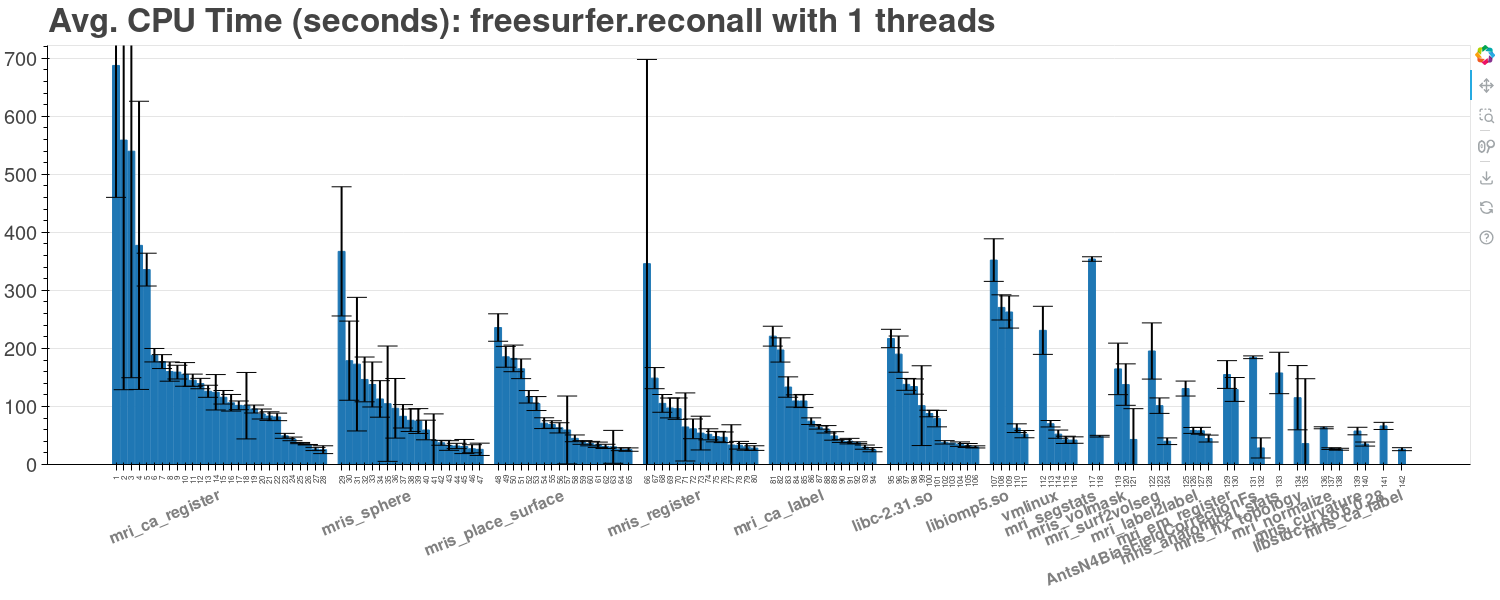
\includegraphics[width=\textwidth]{figures/hotspots-1threads-freesurfer-reconall-simple.png}
	\end{subfigure}
	\begin{subfigure}[t]{0.49\textwidth}
		\caption{Multi-threaded (32 threads)}
		\label{subfig:hotspots-freesurfer-reconall-32threads}
		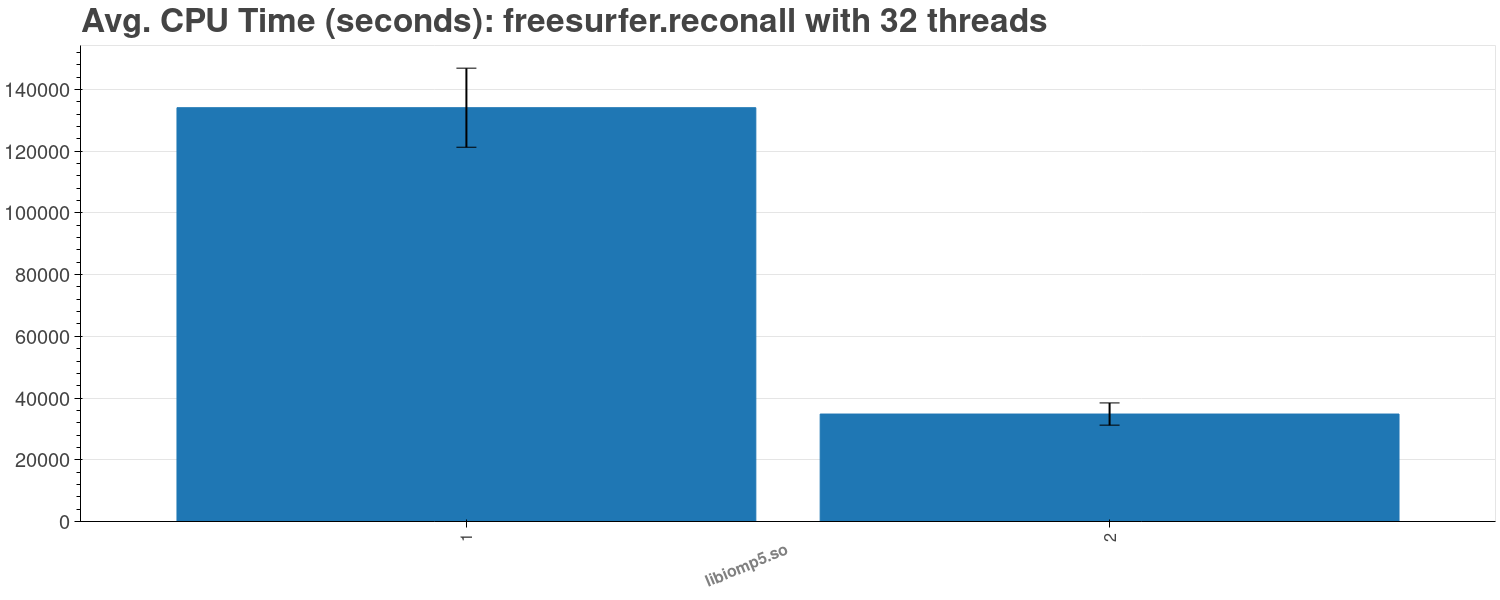
\includegraphics[width=\textwidth]{figures/hotspots-32threads-freesurfer-reconall-simple.png}
	\end{subfigure}
	\caption{FreeSurfer recon-all hotspots analysis. The y-axis show the average CPU time spent in each function, with error bars showing the standard deviation. The x-axis show the function ordered by decreasing CPU time grouped by module. We omit the function names for clarity. The function ID are dependent to each plot. The supplementary materials depicts the mapping of the function ID to the function name for each plot.}
	\label{fig:hotspots-freesurfer-reconall}
\end{figure*}
			
While the makespan for FreeSurfer recon-all decreases with an increase in the number of threads, the benefits are limited (Figure~\ref{fig:freesurfer-threading}). The parallel efficiency decreases from 66\% with two threads down to 5\% with 32 threads. While Amdhals' law plays an impact on the maximum parallel efficiency of the pipeline, Figure~\ref{fig:hotspots-freesurfer-reconall} indicates that the thread Synchronization has a larger impact.
					
\begin{figure}
	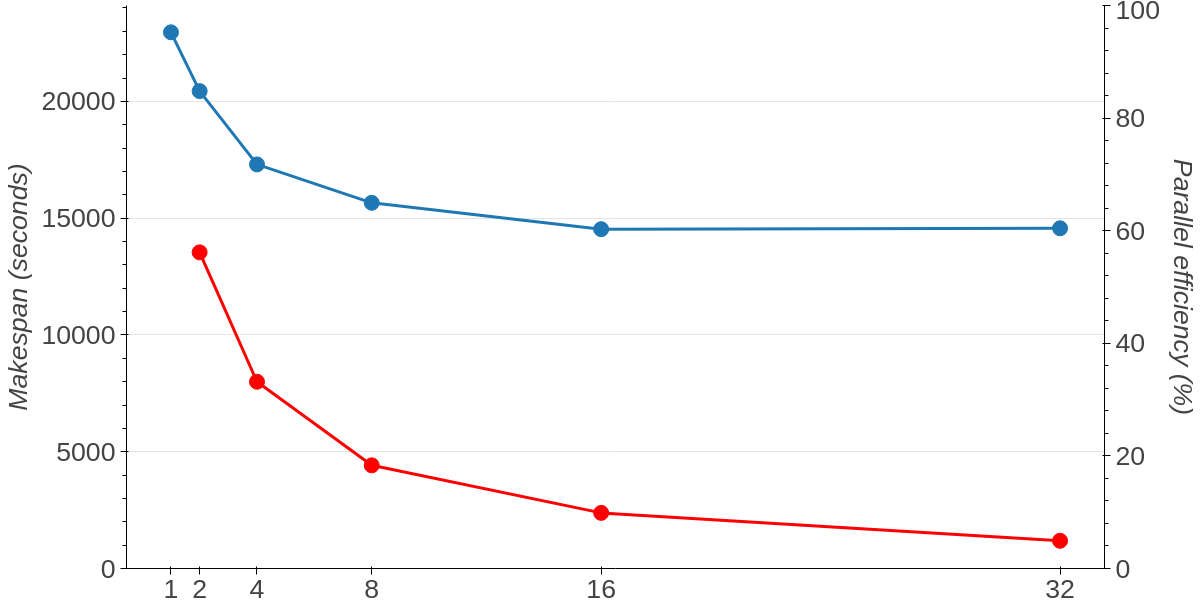
\includegraphics[width=\linewidth]{figures/makespan-freesurfer.png}
	\caption{Makespan and parallel efficiency of FreeSurfer recon-all while varying the number of threads between 1 to 32. The left y-axis shows the makespan in seconds, while the right y-axis shows the parallel efficiency in percent. The log-scaled x-axis shows the number of threads.}
	\label{fig:freesurfer-threading}
\end{figure}
								
\section{Discussion}

\TG{I think the discussion should be merged in the results. I know it's unconventional but I think it would make the paper easier to read and more interestingly. You could add a short conclusion that summarizes the main take-aways from the results.}

\subsection{Few functions account for most of the CPU time}
Our initial assumption was that the distribution of CPU time would follow a Pareto distribution. Thus, 20\% of the functions would contribute to 80\% of the total CPU time. However, Figure~\ref{fig:long-tail-distribution} shows \TG{Figure 2 doesn't ``show'' that. Rephrase.} that the distribution of CPU time is closer to a Zipf's law with exponent $\alpha=1.8$. This means that the CPU time of a function is approximately inversely proportional to its rank. This is consistent with the Pareto's principle, but is more extreme. Therefore, future efforts to optimize the main bottlenecks of MRI pre-processing pipelines could lead to enormous performance improvements.
			
\subsection{Wasted CPU cycles due to Memory Bound}
Overall, our results show a high percent of memory bound across all pipelines.
Optimizing the data access of the application could reduce the number of data load. This would potentially have a large impact on the performance of the pipelines. Alternatively, the use of reduced precision could reduce the memory footprint, thus the memory bound. To reduce the memory bound impact of fetching data from disk, it could be possible to convert and store the data to a lower precision before pre-processing. In both cases, the impact of reduced precision on the accuracy of the pipelines should be studied.
\TG{You could cite some of Valerie's works in this direction.}

\subsection{Importance of Linear Interpolation}
Our results show that linear interpolation the primary bottleneck for all pipelines, except FreeSurfer recon-all. While each interpolation have low computational cost, the large amount of operations make it a significant bottleneck.

There is an extensive literature on interpolation \TG{cite it}. Unfortunately, large amount of optimization techniques are not applicable to MRI pre-processing pipelines, because of the rotation during registration \TG{explain how interpolation is related to registration. In your presentation of fmriprep, explain what registration is and the role it plays in the pipelines.} \TG{this is a bit cryptic and I don't think you want to state that here. You may want to say that it would be interesting to further investigate these techniques in the future.} which requires dynamic kernels for interpolation. Moreover, the high-resolution of the data and iterative refinement of the registration require a large number of interpolations to be performed.

The authors in \cite{Canelhas2018-vs} review different linear interpolation methods ranging from poorly performing nearest-neighbor to classical trilinear interpolation. They review algorithm trade-off accuracy for a lower computational cost. We think it would be interesting for future work to explore these different alternatives to accelerate interpolation within the pipelines. However, special attention will be required to balance the accuracy and the performance of the algorithm.

Similarly, we propose future efforts to explore reduced- or mixed-precision techniques to accelerate interpolation. Optimizing the data format used for interpolation would reduce the computational cost, memory footprint, and storage requirements.

Improvements to interpolation in 3D MRI imaging would have a large impact. It would also benefit other fields of studies using interpolation for high-resolution imaging with iterative refinement, such as climate simulation, astronomical imaging, or 3D image reconstruction. \TG{You could summarize the previous 3 paragraphs, I find them a bit verbose.}

\subsection{ANTS: A tale of precision}
From our results, we observe a slow-down for the single precision version of ANTs pipelines. A single iteration takes longer to execute when using single-precision compared to double precision. After a further analysis of the ANTs registrationSyN single-precision pipeline, we found that the function\footnote{\href{https://github.com/InsightSoftwareConsortium/ITK/blob/d9c585d96359bf304ad3047148cee81bf27ac0c1/Modules/Core/ImageFunction/include/itkVectorInterpolateImageFunction.h\#L46-L48}{itkVectorInterpolateImageFunction.h}} contributing most of the CPU time does computations in double precision. Therefore, the pipeline wastes CPU cycles to convert the input data to double in ITK, and potentially to cast to back to float in ANTS. We think this bug is the cause of the slow-down. We tried recompiling a version of ITK to fix this issue, but we were unsuccessful due to the size and complexity of the code base. This example shows that the use of reduced precision is not trivial and require a deep understanding of the code base. Moreover, benchmark should be performed to ensure that the reduced precision does not impact the performance or accuracy of the pipeline. \TG{Can you report the bug and add a link to the issue here?}

\subsection{OpenMP bottleneck in FreeSurfer recon-all}
In our experiments, FreeSurfer recon-all showed a significant decrease in parallel efficiency with an increase in the number of threads. While Amdhals' law plays an impact on the maximum efficiency, the OpenMP thread synchronization played the largest impact in our results. The codebase uses 83 \textit{static} scheduling policy out of 92 total \TG{explain what these numbers represent}. \textit{Static} scheduling assign chunks to threads in round-robin fashion. This could lead to a load imbalance between the threads, and thus a decrease in parallel efficiency. We speculated that \textit{dynamic} scheduling could improve the parallel efficiency, by assigning chunks based on the current load of the threads. Unfortunately, we failed to recompile FreeSurfer by naively changing the \textit{static} OpenMP scheduling to \textit{dynamic}. This remains challenging as the codebase is large and complex, and the change in scheduling policy could lead to unexpected bugs. \TG{Could you file a bug report in freesurfer on this issue and refer to it here?}
			
Future work should study the different configuration of OpenMP scheduling in FreeSurfer recon-all to improve the parallel efficiency. We believe that significant performance improvements could be achieved by optimizing the thread synchronization. This would lead to faster runtime time and higher CPU usage ration in HPC allocations.
			
\subsection{VTune results finalization}
Using VTune to collect profiling results does not add a large overhead in term of time and resources utilization. However, a finalization step is required to query the data and generate a VTune report. We found this step to be both time consuming and resource intensive. For example, finalizing the results from a single FreeSurfer recon-all execution requires up to \SI{2}{\tera\byte} of RAM, while the developers recommend to use between \SI{8}{\giga\byte} to \SI{16}{\giga\byte} of RAM to run the pipeline. This significant difference in resource requirement creates a challenge to profile pipeline with long runtime, due to the potential difficulty to obtain access to compute nodes with enough RAM. This can be further challenging for researchers in early career or in developing countries, which might not have access to large HPC infrastructure.
One way to mitigate this challenge is to lower the sampling rate during the profiling. However, to reach a similar level of memory consumption, the sampling rate must be significantly reduced. This would lead to a potential loss of information in the profiling results.

\subsection{Limitations}
\TG{You should frame the limitations as future work in the conclusion. These are not really limitations.}
The dataset we chose contains wide range of age and equal distribution of sex. However, it only contains healthy subjects. Therefore, the performance bottleneck we found might not be applicable to data pre-processing of pathological patients. Moreover, the dataset is from a single site. This could also introduce bias from the scanner model and data acquisition protocol used. Future work should include data from multiple sites to ensure the generalization of the performance bottleneck we found. \TG{Is there evidence showing that this would provide additional insights on the benchmark? I think it might be interesting to study subjects that fail QC but I'm not sure about other populations.}
			
Our analysis omits the space or time of execution for function calls \TG{I don't understand what this means}. This information could provide additional insight for optimization. For example, spatial and temporal dimensions were shown to be important in the field of reduced precision. Future work could extent the depth of the analysis by including this information.
\MD{TODO Cite paper on spatial/temporal for RP (ask yohan for references)}
			
\section{Conclusion}
In this paper, we profiled several MRI pre-processing applications: ANTS brainExtraction, ANTS registration, FSL FAST, FSL FLIRT, FSL MCFLIRT, FreeSurfer recon-all, and fMRIPrep. We confirmed our hypothesis \TG{don't frame it as a hypothesis, it is an observation} that few functions contribute to a large amount of CPU time \TG{, which [explain why it is interesting to know]}. We found that most applications suffered from memory bound. Linear interpolation was the primary bottleneck for these applications. We discovered a bug in ITK which lead the implementation of ANTS registration in single-precision to use float for its computation. We also discovered a potential bug in FreeSurfer recon-all which limits the benefit from multi-threading with OpenMP. Last, we discuss the challenge of profiling long running applications with VTune, due to computational resource requirements to obtain results.

We suggest that future effort focus on reduced precision techniques, which could reduce memory bound and accelerate interpolation computation. We note that the use of reduced precision is not trivial, as seen with the ANTS bug. Therefore, careful attention would be required to find a balance between performance and accuracy, while ensuring bugs are not introduced. We also suggest that future work should study the different configuration of OpenMP scheduling in FreeSurfer recon-all to improve the parallel efficiency. This would lead to faster runtime time and higher CPU usage ration in HPC allocations.

We hope that this work serves as a reference for future work to optimize MRI pre-processing pipelines. 
			
			
\section{Data Availability}
\label{sec:data-availability}
The entire OpenNeuro ds004513 v1.0.2 dataset is freely available to download at:
\\\href{https://openneuro.org/datasets/ds004513/versions/1.0.2}{https://openneuro.org/datasets/ds004513/versions/1.0.2}.
	
The container images for our profiling experiments are publicly on Docker Hub:
\begin{itemize}
	\item mathdugre/cmake:debug-info
	\item mathdugre/intel-compilers:debug-info
	\item mathdugre/afni:debug-info
	\item mathdugre/ants:debug-info
	\item mathdugre/fsl:debug-info
	\item mathdugre/freesurfer:debug-info
	\item mathdugre/fmriprep:debug-info
\end{itemize}
	
Our profiling results from VTune are publicly available at:
\\\href{URL}{\MD{TODO add Zenodo link}}
% Waiting on data transfer from Compute Canada
	
\section{Code Availability}
\label{sec:code-availability}
The code to compile, profile the pipelines, and generate figures is publicly available at:
\\\href{https://github.com/mathdugre/mri-bottleneck}{https://github.com/mathdugre/mri-bottleneck}
\MD{TODO Update URL to slashbin org, when created.}
													
\section*{Acknowledgement}
Mathieu Dugr'e was jointly funded by the Natural Sciences and Engineering Research Council of Canada (NSERC) through the Postgraduate Scholarship-Doctoral (PGS-D) program and the Graduate Doctoral Fellowship Award from Concordia University.
\MD{Q: Any other?}
													
\section*{Conflict of Interests}
The authors report no conflict of interests.
													
\bibliographystyle{IEEEtran}
% \bibliography{IEEEabrv, paper}
\bibliography{paper}
													
\newpage
\onecolumn
\section*{Supplementary Materials}
\MD{Not sure if these add value?}
\label{sec:supplementary}

\begin{figure*}[ht]
	\centering
	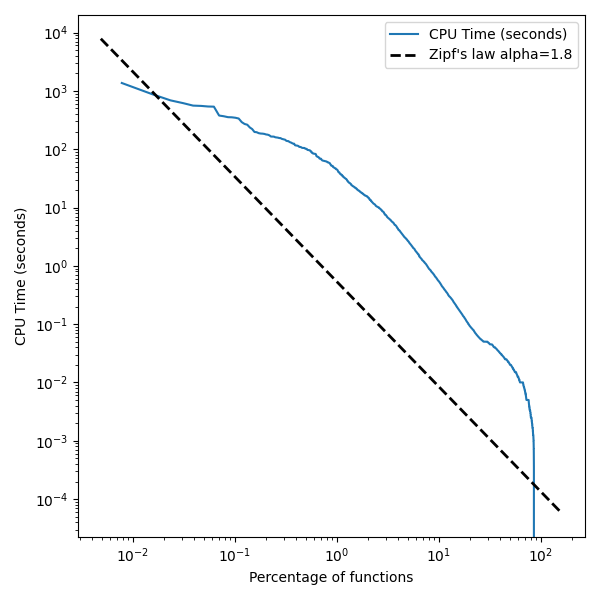
\includegraphics{figures/global-zipf_law.png}
	\caption{Distribution of the functions' CPU time compare to a Zipf's law distribution with $\alpha=1.8$. The y-axis shows the average CPU time for a function. The x-axis shows the percentage of functions ordered by decreasing CPU time. The data includes all functions from all pipelines.}
	\label{sup-fig:zips-law}
\end{figure*}
													
\csvnames{csvcol}{2=\module, 3=\func, 4=\mean, 5=\std}
\csvstyle{hotspot}{
	tabular = |r|l|l|c|,
	table head = \hline & Module & Function & CPU Time (mean$\pm$std)\\\hline\hline,
	late after line = \\\hline,
	respect all,
	csvcol
}
\newcommand{\csvtable}[3]{
	\begin{table}[ht]
		\resizebox*{\textwidth}{!}{
			\csvreader[hotspot]{#1}{}
			% \csvreader[hotspot, filter={\value{csvrow}<60}]{#1}{}
			{\thecsvrow & \module & \func & \tablenum[round-precision=2, round-mode=places]{\mean}$\pm$\tablenum[round-precision=2, round-mode=places]{\std}}
		}
		\caption{#2}
		\label{#3}
	\end{table}
}
% CSV tables
% \csvtable{tables/hotspots-1thread-freesurfer-reconall.csv}{FreeSurfer recon-all (1 thread): Top functions accouting for 80\% of the application makespan.}{extab:hotspots-1thread-freesurfer-reconall}
\csvtable{tables/hotspots-32threads-freesurfer-reconall.csv}{FreeSurfer recon-all (32 threads): Top functions accouting for 80\% of the application makespan.}{extab:hotspots-32threads-freesurfer-reconall}
			
\end{document}
